%% -*- coding:utf-8 -*-
\author{Stefan Müller}\institute[HU Berlin, Institut für deutsche Sprache und Linguistik, Syntax]{}

\settowidth\jamwidth{(Niederländisch)}

\subtitle{Phänomene}

\section{Phänomene}

\huberlintitlepage[22pt]

\outline{

\begin{itemize}
\item {Überblick über die germanischen Sprachen}
\item \alert{Phänomene}
\item Phrasenstrukturgrammatiken und \xbart
\item Valenz, Argumentanordnung und Adjunkte
\item Verbalkomplexbildung in den SOV-Sprachen
\item Verbstellung: Verberst- und Verbzweitstellung
\item Passiv
\item Eingebettete Sätze
\end{itemize}

}



\frame{
\frametitle{Übungsaufgaben/Wiederholung}


Bestimmen Sie in den folgenden Sätzen die topologischen Felder, die Wortarten der Wörter, die Kasus der Nominalgruppen und die
grammatischen Funktionen und zeichnen Sie für einen Satz einen Strukturbaum in einem theoretischen
Modell Ihrer Wahl (\zb Government \& Binding)!
\eal
\ex Der Mann lacht.
\ex Der Frau hat der Mann das Buch gegeben, den wir kennen.
\ex Ein Lied singend ging Peter voran.
\ex Einen Aufsatz schreiben, der komplett neue Gedanken enthält,\\
    können nur wenige.
\zl

}

\frame{
\frametitle{Literaturhinweis}


Grundbegriffe (Wortarten, grammatische Funktionen, topologische Felder, \ldots): Kapitel~1 in \citew{MuellerGT-Eng}.
\begin{refsection}

\nocite{MuellerGT-Eng}

\printbibliography[heading=none,notkeyword=this]

\end{refsection}

\pause

Zu Phänomenen im Germanischen: Kapitel~2 in \citew{MuellerGermanic}.


\begin{refsection}

\nocite{MuellerGermanic}

\printbibliography[heading=none,notkeyword=this]

\end{refsection}





}


  


\frame{
\frametitle{Variation}

\begin{itemize}
\item Stellung:
\begin{itemize}
\item VO vs.\ OV
\item V2 vs. Nicht-V2
\item Anordnung von Subjekten und Objekten (fest oder umstellbar)
\item Stellung der Adverbien
\end{itemize}
\item Verbalkomplexe
\item Subjektbedingung
\item Passiv
\begin{itemize}
\item persönliches Passiv
\item unpersönliches Passiv
\item Objekte ditransitiver Verben
\end{itemize}
\item Expletivpronomina
\begin{itemize}
\item Markierung Satztyp in nicht eingebetteten Sätzen (V2)
\item Markierung Satztyp in eingebetteten Sätzen (V3)
\end{itemize}
\end{itemize}


}


\subsection{Warnung: OV/VO vs.\ V2/Nicht-V2}

\frame{
\frametitle{Warnung: OV/VO vs.\ V2/Nicht-V2}

\begin{itemize}
\item Sprachen werden nach Abfolge von Subjekt, Objekt und Verb in Klassen eingeteilt:
\begin{itemize}
\item SOV
\item SVO
\item \ldots
\end{itemize}
\item Das heißt nicht, dass alle Sätze einer Sprache immer diesem Muster entsprechen.
\item Es sagt etwas über den Sprachtyp aus.

\item Die Eigenschaft, eine V2-Sprache zu sein oder nicht, ist davon unabhängig.

\item Dritte, prinzipiell unabhängige Eigenschaft:\\
      Umordenbarkeit des Subjekts und der Objekte (Scrambling).

\item \citet{Haftka96a}:\\
      \emph{Deutsch ist eine V/2-Sprache mit Verbendstellung und freier Wortfolge}

Klingt wie einer, ist aber kein Widerspruch.

\end{itemize}
}


\subsection{Abfolge von Subjekt, Objekt und Verb}

\frame[shrink]{
\frametitle{Subjekt, Objekt und Verb in den Sprachen der Welt}

\medskip

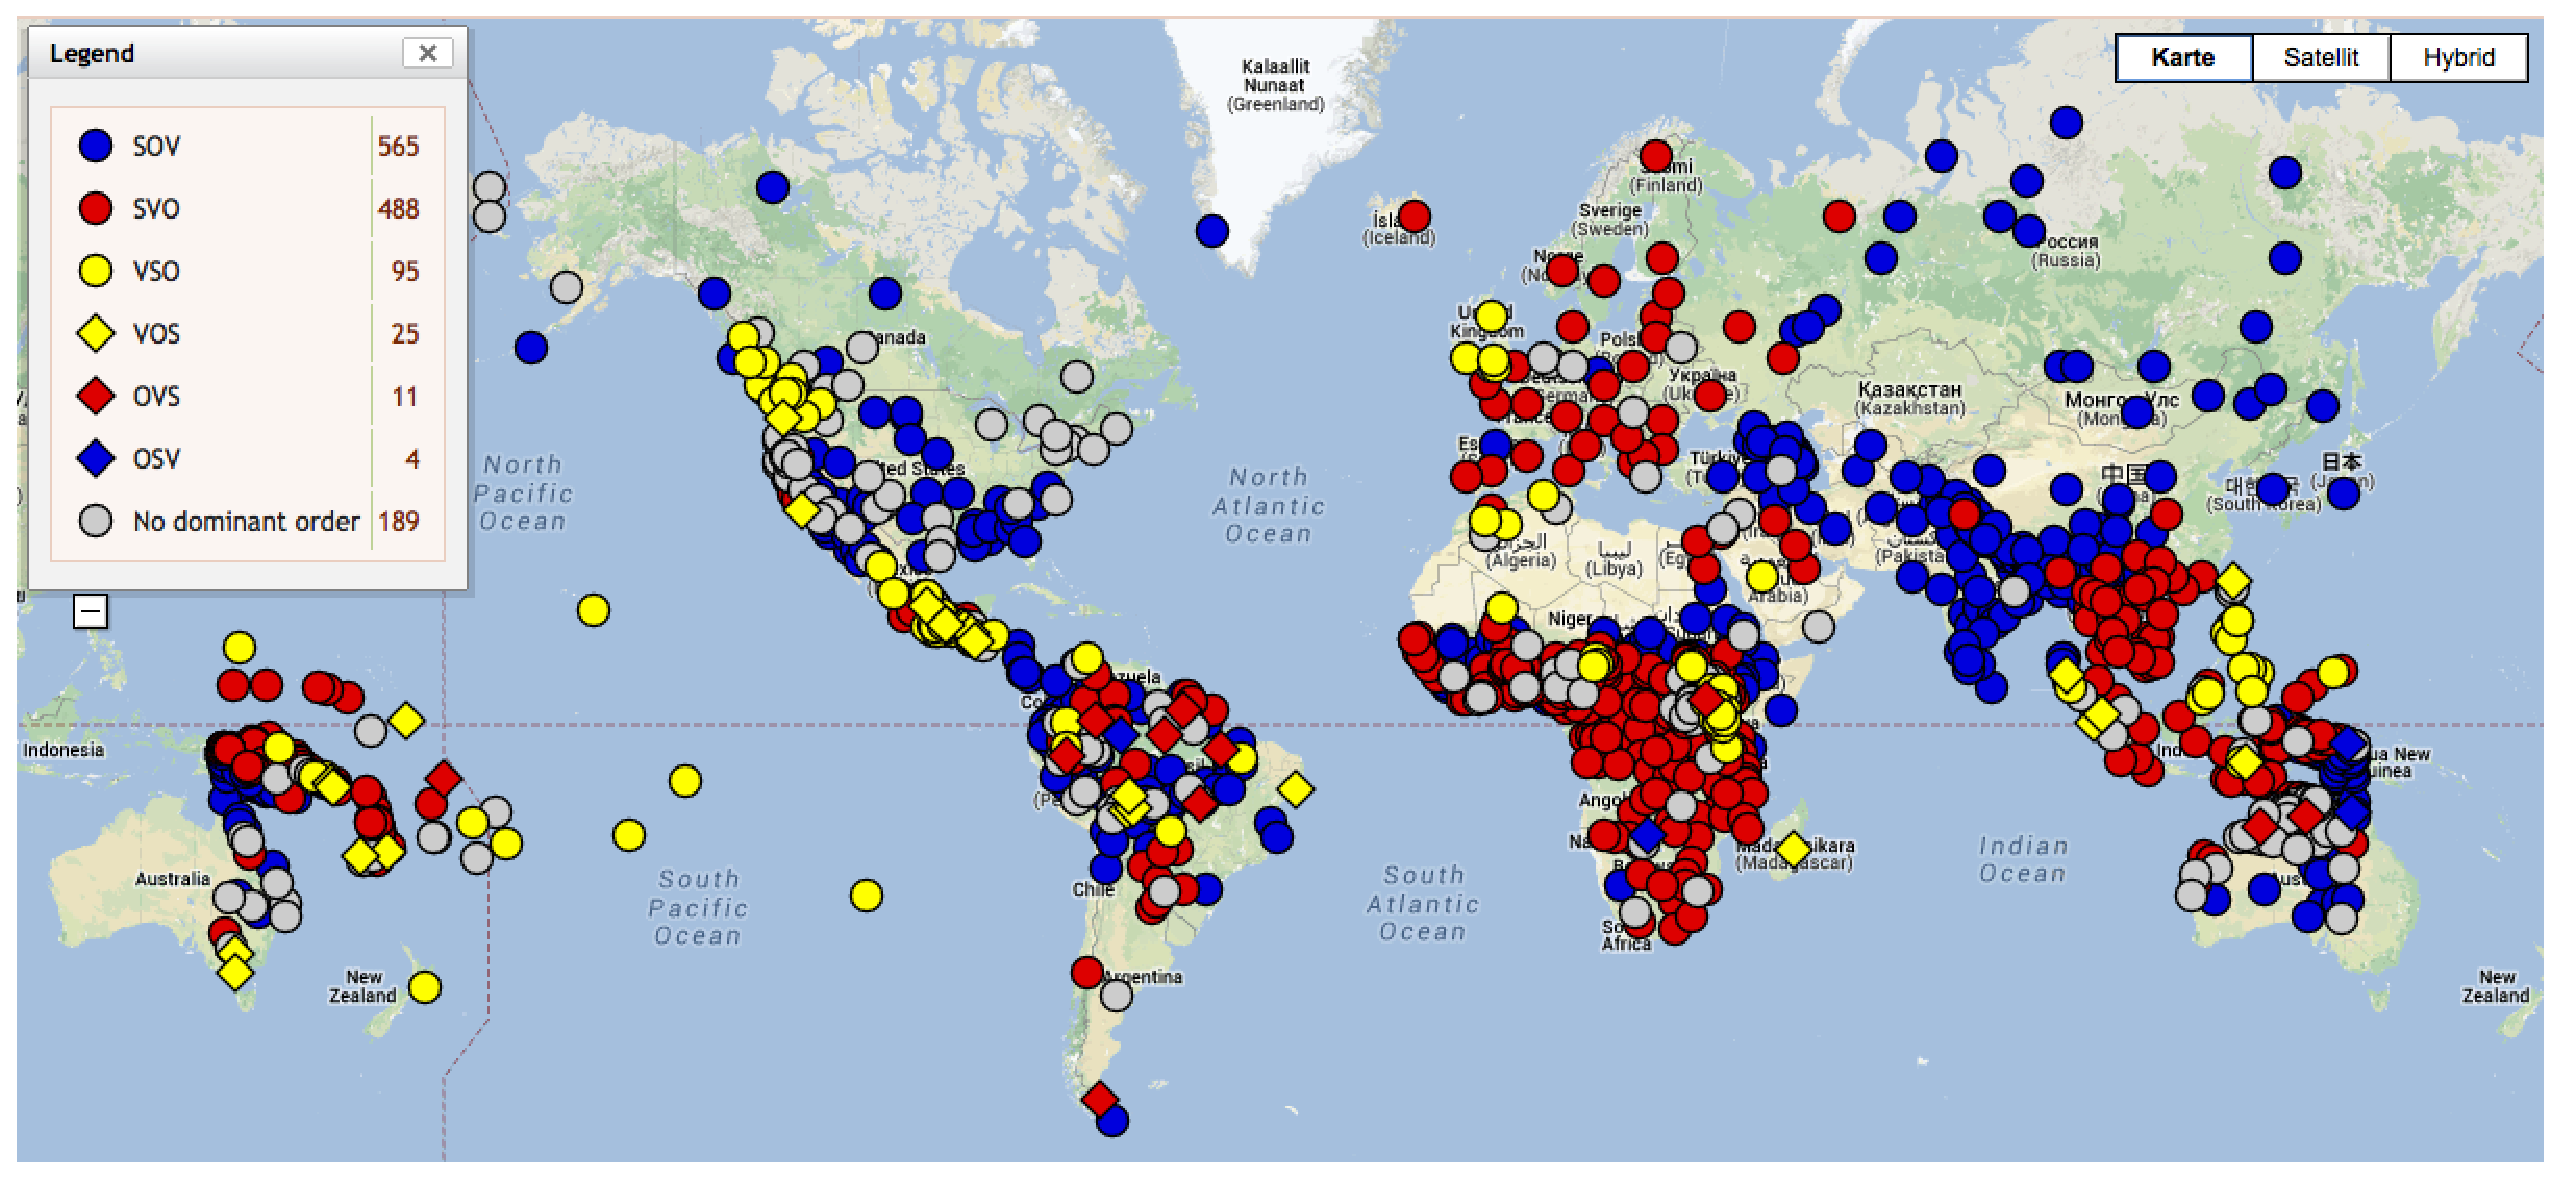
\includegraphics[width=\textwidth]{Bilder/WALS-SOV}

\vfill

{\small Matthew S. Dryer: Feature 81A: Order of Subject, Object and Verb,\\
 The World Atlas of Language Structures} 


}

\frame{
\frametitle{Subjekt, Objekt und Verb im WALS}

\begin{itemize}
\item Subjekte sind die Argumente mit den eher agensartigen Eigenschaften.
\pause
\item Objekte sind die Argumente mit den eher patiensartigen Eigenschaften.
\pause
\item Das ist nicht unbedingt deckungsgleich mit einzelsprachlichen Definitionen von Subjekt.
\ea
Der Aufsatz interessiert mich.
\z
\item Dominante Abfolge (Dryer: Determining Dominant Word Order):

Where a language is shown on one of the word order maps as having a particular order as the dominant
order in the language, this means that it is either \blaubf{the only order possible} or the order
that is \blaubf{more frequently used}.


I base my classification of Macushi here on the frequency counts, and since no order is more than
twice as frequent as the next most frequent order, I treat this language as lacking a dominant order
of subject, object, and verb.


Deutsch, Niederländisch und Friesisch sind V2-Sprachen, \dash die SVO- und SVAuxOV-Stellungen kommen
durch die Voranstellung des Verbs zustande, die eine Funktion hat. Wir zählen diese Sprachen also
mit zu den SOV-Sprachen.

\end{itemize}



}

\frame{
\frametitle{Subjekt, Objekt, Verb in Europa}

\begin{columns}[T]
\begin{column}{90mm}
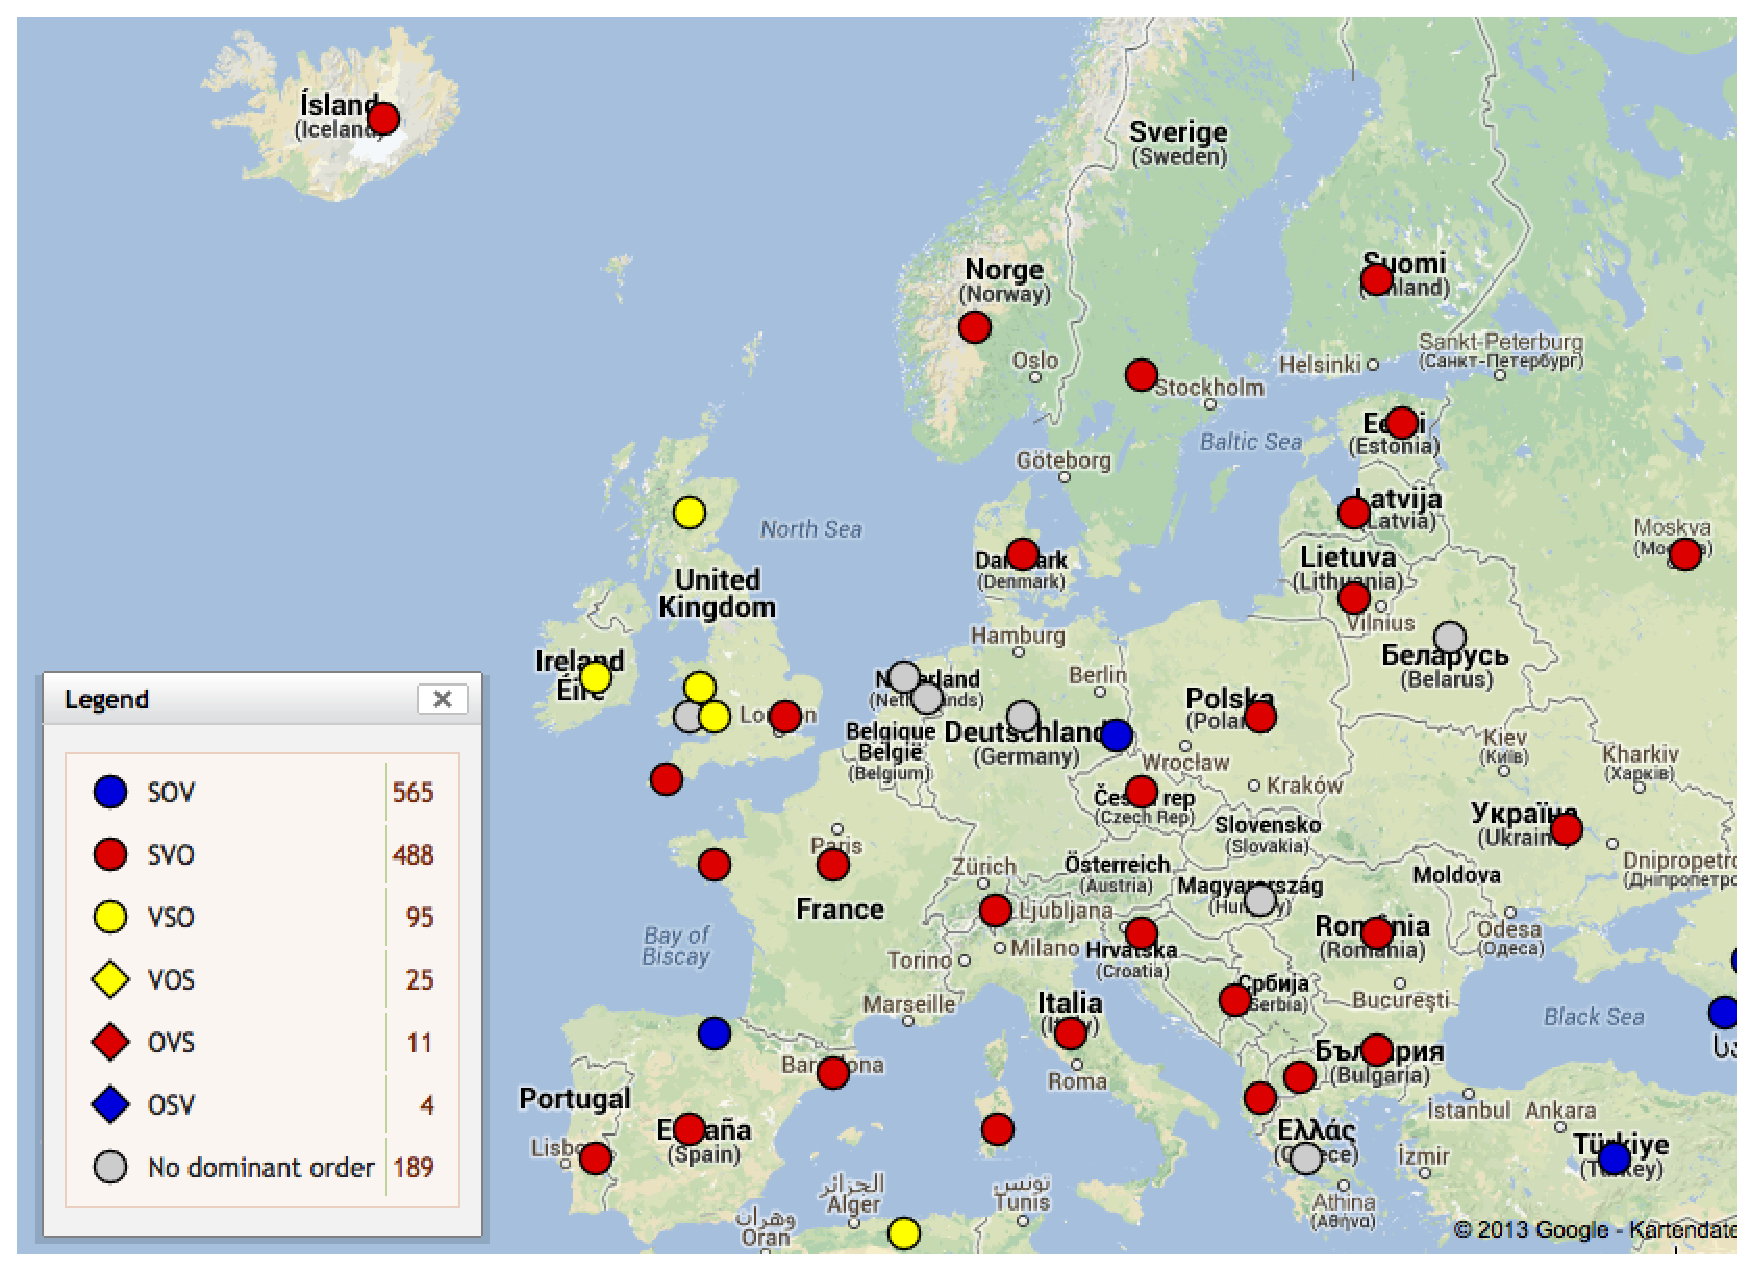
\includegraphics[width=\textwidth]{Bilder/WALS-SOV-Europa}
\end{column}
\begin{column}{25mm}
SVO:\\
Isländisch,\\
Norwegisch,\\
Schwedisch,\\
Dänisch,\\
Englisch
\end{column}
\end{columns}
}


\frame{
\frametitlefit{Dryer: Feature 81b: Two Dominant Orders of Subject, Object, and Verb}

\begin{columns}[T]
\begin{column}{90mm}
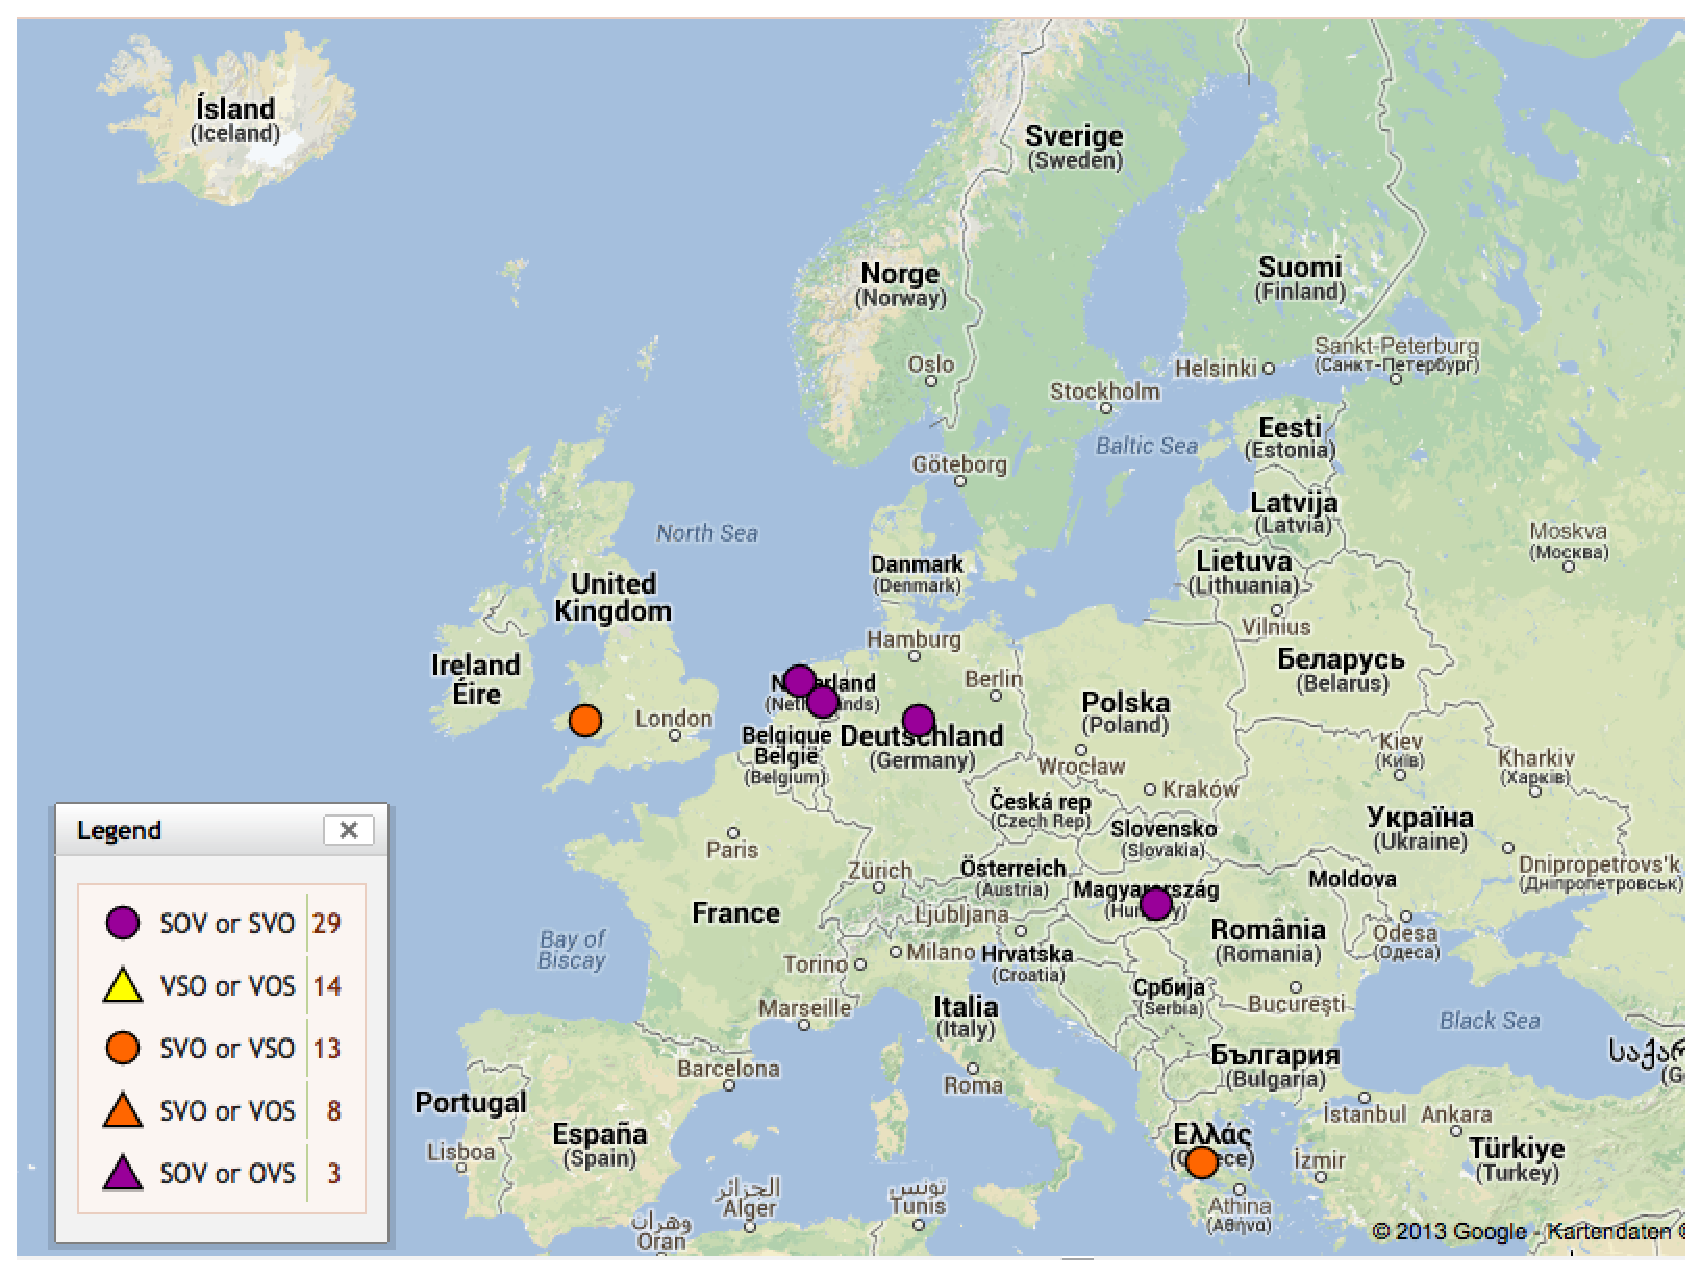
\includegraphics[width=.95\textwidth]{Bilder/WALS-SOV-Europa-no-dominant}
\end{column}
\begin{column}{30mm}
SVO oder SOV:\\
Deutsch,\\
Friesisch,\\
Niederländisch
\end{column}
\end{columns}
% Walisisch: SVO oder VOS
% Friesisch
% Niederländisch
% Deutsch 
% Ungarisch

}
% Eisenberg89:409 zitiert Greenberg66 mit Deutsch als SVO.


\frame{
\frametitle{Sprachen ohne dominante Konstituentenstellung im WALS}

Dryer:

A third subtype of language lacking a dominant order consists of languages in which different word
orders occur but the choice is syntactically determined. For example, in \blaubf{German and Dutch}, the
dominant order is \blaubf{SVO in main clauses lacking an auxiliary} and \blaubf{SOV in subordinate clauses and
clauses containing an auxiliary} [\ldots]. Because this results in both orders being
common, neither order is considered dominant here and these two languages are shown on the map as
lacking a dominant word order. In general, if the word order varies according to whether there is an
auxiliary verb, the language is shown on the map as lacking a dominant order.


}

\frame{
\frametitle{Hilfsverben zählen nicht, or do they?}

\eal
\ex Kim sieht den Fuchs.
\ex Kim hat den Fuchs gesehen.
\zl
Für Dreyer ist (\mex{0}a) SVO und (\mex{0}b) SAuxOV.\\
Aux wird ignoriert, so dass das Muster als SOV zählt.
\pause

Aber was ist mit (\mex{1})?
\eal
\ex Kim scheint den Fuchs zu sehen. \hfill(SVOV?)
\pause

\ex Kim scheint den Fuchs gesehen zu haben.
\zl

Es ist einfach das finite Verb, das aus Gründen der Satztypmarkierung anders plaziert wird.


}

\frame[shrink=5]{
\frametitle{OV vs.\ VO}

OV: Verben stehen nach dem Objekt:

\eal
\ex dass sie ihn sieht$_1$   \jambox{(Deutsch, SOV)}
\ex dass sie ihn gesehen$_2$ hat$_1$
\ex dass sie ihn gesehen$_3$ haben$_2$ muss$_1$
\zl

Einbettende Verben werden nach eingebetteten angeordnet.

\pause

VO: Verben stehen vor dem Objekt:

\eal
\ex
\gll at   hun ser$_1$ ham\\
     dass sie  sieht   ihn\\\jambox{(Dänisch, SVO)}
\ex
\gll at   hun have$_1$ set$_2$ ham\\
     dass sie  hat      gesehen ihn\\
\ex
\gll at hun må$_1$ have$_2$ set$_3$ ham\\
     dass sie muss haben gesehen ihn\\
\zl

OV: Deutsch, Niederländisch, Afrikaans, \ldots

VO: Englisch, Dänisch, Norwegisch, Schwedisch, \ldots

}

\frame{
\frametitle{Partikelverben und Resultativkonstruktionen}

%[Section~15.2]
\citet{Haider2020a}: Weitere Unterschiede zwischen VO- und OV-Sprachen:

Partikelverben:
\eal
\ex Kim will \alert{look up} the information.      \hfill(Verb < Partikel)
\ex Kim wird die Information \alert{nachschlagen}. \hfill(Partikel < Verb)
\zl
\pause

Resultativkonstruktionen:
\eal
\ex Kim will \alert{fish} the pond \alert{empty}.       \hfill(Verb < Pred)
\ex Kim wird den Teich \alert{leer} \alert{fischen}.    \hfill(Pred < Verb)
\zl



}

\subsection{V2}

\frame{
\frametitle{V2}

\begin{itemize}
\item Das Deutsche ist eine V2-Sprache:\\
      Das finite Verb steht in Aussagesätzen und \emph{w}"=Fragen an zweiter Stelle.
\item Davor kann eine beliebige Konsitutente stehen:
\eal
\ex Das Kind  gibt dem Eichhörnchen jetzt eine Nuss.
\ex Dem Eichhörnchen gibt das Kind jetzt eine Nuss.
\ex Eine Nuss gibt das Kind dem Eichhörnchen jetzt.
\ex Jetzt gibt das Kind dem Eichhörnchen eine Nuss.
\zl
\eal
\ex Wer gibt dem Eichhörnchen jetzt eine Nuss?
\ex Wem gibt das Kind jetzt eine Nuss?
\ex Was gibt das Kind dem Eichhörnchen jetzt?
\ex Wann gibt das Kind dem Eichhörnchen eine Nuss?
\zl
\end{itemize}

}

\frame{
\frametitle{V2 vs.\ Nicht-V2}

\begin{itemize}
\item Bis auf das Englische sind die germanischen Sprachen V2-Sprachen:
\eal
\ex Bagels mag ich.\jambox{(Deutsch)}
\ex Bagels, I like.\jambox{(Englisch)}
\zl 


\eal
\ex Gestern gab ich dem Eichhörnchen eine Nuss.\jambox{(Deutsch)}
\ex Yesterday, I gave the squirrel a nut.\jambox{(Englisch)}
\zl 

\item Es gibt Voranstellung im Englischen, diese erfolgt aber immer vor das Subjekt und das Verb.

\end{itemize}

}

\frame{
\frametitle{Nicht extrahierbare Elemente}

In den V2-Sprachen können fast alle Argumente vorangestellt werden. 

Im Englischen (sprecherabhängig) nicht alle Objekte voranstellbar \citep[\page 258]{Hudson92a-u}:

\eal
\judgewidth{\%}
\ex[]{
We give children sweets.
}
\ex[]{
These sweets, we give children \_.
}
\ex[\%]{
These children, we give \_ sweets.
}
\zl

}

\frame{
\frametitle{Voranstellung über Satzgrenzen hinweg}



\ea
{}[Über dieses Thema]$_i$ habe ich sie gebeten, [[einen Vortrag \_$_i$~] zu halten]?\footnote{
Nach \citew[\page 21]{HN89b}.
}
\z

Analyse von V2 kann also nicht einfach Umstellung von Satzgenossen sein.


}


\frame{
\frametitle{V2 und OV/VO}

\begin{itemize}
\item V2 ist unabhängig von VO/OV. Dänisch ist SVO und V2.
\eal
\ex 
\gll Gert har læst bogen.\\
     Gert hat gelesen Buch.{\sc def}\\\jambox{(Dänisch)}
\ex
\gll Bogen har Gert læst.\\
     Buch.{\sc def} hat Gert gelesen\\\jambox{(Dänisch)}
\zl


\end{itemize}

}

\frame{
\frametitle{Englisch als Residual V2}

Im Englischen gibt es Reste von V2-Strukturen in Fragen:
\eal
\ex Which book did Sandy read?
\ex Which book did Sandy give to Kim?
\ex To whom did Sandy give the book?
\zl

\citet[\page 375]{Rizzi1990a-u}:  \emph{residual V2 language}



}


\frame{
\frametitle{Satztypen}

Satztypen werden über Verbstellung kodiert. Neben Aussagesätzen und \emph{w}-Fragesätzen gibt es
auch V2-Imperative:

\ea
Jetzt gib ihr das Buch!
\z
\pause

Ansonsten: Entscheidungsfragen und Imperative als V1:
\eal
\ex Gibt er ihr das Buch?
\ex Gib ihr das Buch!
\zl

} 


\frame{
\frametitle{V2 ist selten}

V2 ist selten \citep[\page 343]{Holmberg2015a}.

\begin{itemize}
\item germanische Sprachen (außer Englisch, \citealp{HP86a-ed})
\item modernes Bretonisch \citep{BK2000a-u}
\item Estnisch
\item Altfranzösisch \parencites[Section~1.3]{Adams1987a-u}[Section~2.1.2]{Roberts93a-u}[Chapter~2]{Vance97a-u},
  Altitalienisch, Altspanisch \citep[Section~3.3.2]{Fontana97a-u}, 
\item Rätoromanisch \citep{Poletto2002a-u,Anderson2006a-u},
\item das Kashmiri (Indien, Pakistan, \citealp[Chapter~4]{Bhatt99a-u})
\item Inguschisch (autonomen Republik Inguschetien, Russische Föderation)
\item die austronesischen Sprachen Taiof und Sisiqa, \citep[\page 495]{Ross2004a-u} % wieder aus der englischen Wikipedia verschwunden
\item die Sprache brasilianischer Ureinwohner*innen Karitiana aus der Tupí-Familie \citep{Storto2003a-u} 
% Ist vielleicht nur X2 sowas wie die australischen Sprachen (Bayer2010)
%\item die uto-aztekische Sprache Tohono O'odham\\
%      (Südwesten der USA sowie im Norden Mexikos).
\end{itemize}



}





\subsection{Scrambling}

\frame{
\frametitle{Scrambling oder nicht}

Germanische OV-Sprachen (Deutsch, \ldots):\\
prinzipiell alle Abfolgen von Argumenten möglich:
\eal
\ex {}[weil] \rot{das Kind} \gruen{dem Eichhörnchen} \blau{die Nuss} gibt
\ex {}[weil] \rot{das Kind} \blau{die Nuss} \gruen{dem Eichhörnchen} gibt
\ex {}[weil] \blau{die Nuss} \rot{das Kind} \gruen{dem Eichhörnchen} gibt
\ex {}[weil] \blau{die Nuss} \gruen{dem Eichhörnchen} \rot{das Kind} gibt
\ex {}[weil] \gruen{dem Eichhörnchen} \rot{das Kind} \blau{die Nuss} gibt
\ex {}[weil] \gruen{dem Eichhörnchen} \blau{die Nuss} \rot{das Kind} gibt
\zl

\pause

Germanische VO-Sprachen (Englisch, \ldots): Argumente haben eine feste Stellung.
\eal
\ex because \rot{the child} gives \gruen{the squirrel} \blau{the nut}
\ex because \rot{the child} gives \blau{the nut} \gruen{to the squirrel} 
\zl
\emph{Dative Shift} erfordert Umkategorisierung. Markierung durch Präposition.


}

\subsection{Stellung der Adverbialien}

\frame{
\frametitle{Stellung der Adverbialien}


Deutsch, Niederländisch, \ldots: Stellung der Adverbien frei:
\eal
\ex weil das Kind dem Eichhörnchen die Nuss \blauit{gestern} gab
\ex weil das Kind dem Eichhörnchen \blauit{gestern} die Nuss gab
\ex weil das Kind \blauit{gestern} dem Eichhörnchen die Nuss gab
\ex weil \blauit{gestern} das Kind dem Eichhörnchen die Nuss gab
\zl

\pause

Dänisch, Englisch, \ldots: Adverbien stehen vor oder nach der VP:
\eal
\ex because the child \blauit{often} [\gruen{gave the squirrel the nut}]
\ex because the child [\gruen{gave the squirrel the nut}] \blauit{often}
\zl

\pause
Extremfall verschachtelte VPen \citep[§ 8.20, 495]{QGLS85a-u}:
\ea
It [\blauit{certainly} [\sub{VP} may [\blauit{possibly} [\sub{VP} have [\blauit{indeed} [\sub{VP} been\\ {}[\blauit{badly} [\sub{VP} formulated]]]]]]]].
\z

}


\subsection{Eingebettete Sätze}

\subsubsection{Konjunktional eingeleitete Nebensätze}

\frame{
\frametitle{Deutsch: eingebettete Sätze sind VL}

\begin{itemize}
\item Deutsch, Niederländisch, \ldots: V-letzt:

\ea
Ich weiß, dass Aicke das Buch heute gelesen hat.
\z

\pause
Stellung der anderen Konstituenten ist frei:
\eal
\ex Ich weiß, dass das Buch Aicke heute gelesen hat.
\ex Ich weiß, dass das Buch heute Aicke gelesen hat.
\zl

\end{itemize}

}

\frame{
\frametitle{Englisch: eingebettete Sätze SVO}


\begin{itemize}
\item Englisch: eingebettete Sätze SVO
\ea[]{
I  know that Kim has read the book yesterday.
}
\z

%% \pause
%% Andere Stellungen sind nicht möglich:
%% \eal
%% \ex[*]{
%% I know that has Max read the book yesterday.
%% }
%% \ex[*]{
%% I know that yesterday Max has read the book.
%% }
%% \zl

\end{itemize}

}



\frame{
\frametitle{Dänisch: eingebettete Sätze SVO oder V2}


\begin{itemize}
\item Dänisch: eingebettete Sätze SVO oder V2
\ea[]{
\gll Jeg  ved, at   Gert ikke  har læst  bogen          {i dag}.\\
     ich weiß dass Gert nicht hat gelesen Buch.{\sc def} heute\\\jambox{(SVO)}
}
\z
Negation hilft, Verbstellung zu bestimmen:
\ea[]{
\gll Jeg  ved, at   Gert har ikke  læst  bogen          {i dag}.\\
     ich weiß dass Gert hat nicht gelesen Buch.{\sc def} heute\\\jambox{(V2)}
}
\z



\pause
Andere Konstituenten in Initial-Stellungen sind möglich, \dash klares V2:
\eal
\ex[]{
\gll Jeg  ved, at   {i dag} har Gert ikke læst bogen.\\
     ich weiß dass heute   hat Gert nicht gelesen Buch.{\sc def}\\
}
\ex[]{
\gll Jeg ved, at   bogen          har Gert ikke  læst {i dag}.\\
     ich weiß dass Buch.{\sc def} hat Gert nicht gelesen heute\\
}
\zl

%% \ex[*]{
%% \gll Jeg  ved, at   {i dag} Gert har læst bogen.\\
%%      ich weiß dass heute   Gert hat gelesen Buch.{\sc def}\\
%% }
%%
%% \ex[*]{
%% \gll Jeg  ved, at   bogen          Gert har læst {i dag}.\\
%%      ich weiß dass Buch.{\sc def} Gert hat gelesen heute\\
%% }
%% \zl

\end{itemize}

}


\frame{
\frametitle{Jiddisch, Isländisch: eingebettete Sätze sind V2}

% Isländisch: Wikipedia (en)

\begin{itemize}
\item Jiddish: eingebettete Sätze sind V2 \citep[]{Diesing90a}:
\eal
\ex
\gll Ikh meyn  az   haynt hot Max geleyent dos bukh.\footnotemark\\
     ich   denke dass heute hat Max gelesen   das Buch\\
\footnotetext{\citew[\page 58]{Diesing90a}.}
\glt `Ich denke, dass Max heute das Buch gelesen hat.'

\ex% check!
\gll Ikh meyn  az   dos bukh hot Max geleyent.\\
     ich denke dass das Buch hat Max gelesen\\

\zl

\pause
Isländisch:
\ea 
\gll Engum         datt í hug,  að   vert  væri að reyna til     að kynnast honum.\footnotemark\\
     no.one.\DAT{} fell to mind that worth was  to try   \PREP{} to know    him\\\icelandic
\footnotetext{\citew[\page 75]{Maling90a-u}.}
\glt `It didn't occur to anyone that t was worth trying to get to know him.'
\z



\end{itemize}

}


\subsubsection{Interrogativnebensätze}


\frame{
\frametitle{Deutsch: Interrogativnebensätze \emph{w} + VL}

\begin{itemize}
\item Deutsch, Niederländisch, \ldots: \emph{w} + V-letzt:

\eal
\ex Ich weiß, wer heute das Buch gelesen hat.
\ex Ich weiß, was Aicke heute gelesen hat.
\zl

Interrogativnebensätze beginnen mit einer \emph{w}-Phrase.

\pause
\item Die \emph{w}-Phrase kann von weit her kommen:
\ea
Ich weiß nicht, [\gruen{über welches Thema}]$_i$ sie versprochen hat,\\
{}[[einen Vortrag \_$_i$] zu halten].
\z

\pause
\item Stellung der anderen Konstituenten ist frei:
\eal
\ex Ich weiß, was keiner diesem Eichhörnchen geben würde.
\ex Ich weiß, was diesem Eichhörnchen keiner geben würde.
\zl



\end{itemize}

}

\frame{

\frametitle{Dänisch, English: Interrogativnebensätze  \emph{w} + SVO}


\begin{itemize}
\item Dänisch: Interrogativnebensätze sind \emph{w} + SVO

\eal
\ex
\gll Jeg ved, hvad Gert har givet ham.\\
     ich weiß was Gert  hat gegeben ihm\\
\glt `Ich weiß, was Gert ihm gegeben hat.'
\ex
\gll Jeg ved, hvem Gert har givet   bogen.\\
     ich weiß wem  Gert hat gegeben Buch.{\sc def}\\
\glt `Ich weiß, wem Gert das Buch gegeben hat.'
\zl

\end{itemize}

}

\frame{
\frametitle{Jiddish: Interrogativnebensätze \emph{w} + V2}

\begin{itemize}
\item Jiddish: Interrogativnebensätze \emph{w} + V2 \citep[Abschnitte~4.1, 4.2]{Diesing90a}

%% \ea
%% %\ex
%% \label{vosmaks}
%% \gll Ikh veys nit   [vos Max hot gegesn].\footnotemark\\
%%      ich weiß nicht \hspaceThis{[}was Max hat gegessen\\
%% \footnotetext{\citew[S.\,68]{Diesing90a}.}
%% \glt `Ich weiß nicht, was Max gegessen hat.'

%% %% \ex%check
%% %% \gll Ikh veys nit   [vos              hot Max gegesn].\footnotemark\\
%% %%      ich weiß nicht \hspaceThis{[}was heute hat Max gegessen\\
%% %% \footnotetext{\citew[S.\,68]{Diesing90a}.}
%% %% \glt `Ich weiß nicht, was Max heute gegessen hat.'


\ea
\gll Ir veyst efsher [avu            do    voynt Roznblat   der goldshmid]?\footnotemark\\
     Sie wissen vielleicht  \spacebr{}wo da wohnt Roznblat der Goldschmied\\
\glt `Wissen Sie vielleicht, wo Roznblat der Goldschmied wohnt?' 
\footnotetext{
\citew[S.\,65]{Diesing90a}. Zitiert aus Olsvanger, \emph{Royte Pomerantsn}, 1949
}
\z
\end{itemize}

}



\subsection{Expletiva zur Satztypmarkierung}

\frame{
\frametitle{Expletiva zur Satztypmarkierung}

\begin{itemize}
\item Germanische Sprachen benutzen Expletiva, um Satztypen kenntlich zu machen,
      falls keine andere Konstituente die entsprechende Position füllt.
\pause
\item Deutsch V2-Hauptsätze

\eal
\ex Drei Reiter ritten zum Tor hinaus.
\ex \rot{Es} ritten drei Reiter zum Tor hinaus.
\zl
\end{itemize}


}

\frame{
\frametitle{Dänisch: \emph{w}-Sätze mit extrahiertem Subjekt}

\begin{itemize}
\item Dänisch: \emph{w} + SVO\\
      Bei Subjektextraktion muss Extraktion explizit kenntlich gemacht werden:
\eal
\ex[]{
\gll Politiet ved ikke, \gruen{hvem} \rot{der}   havde placeret bomben.\\
     Polizei.{\sc def} weiß nicht wer {\sc expl} hat plaziert Bombe.{\sc def}\\
\glt `Die Polizei weiß nicht, wer eigentlich die Bombe plaziert hat.'
}
\ex[*]{
\gll Politiet ved ikke, \gruen{hvem} havde placeret bomben.\\
     Polizei.{\sc def} weiß nicht wer hat plaziert Bombe.{\sc def}\\
}
\zl

\pause

Expletivum macht Extraktion sichtbar:
\eal
\ex[*]{ 
\gll [\gruen{hvem}$_i$     [\trace$_i$ havde placeret bomben]]\\
     \spacebr{}wer {}          hat   plaziert Bombe.\textsc{def}\\\danish
}
\ex[]{
\gll [\gruen{hvem}$_i$     [\rot{der}                    havde \trace$_i$ placeret bomben]]\\
     \spacebr{}who \spacebr{}\textsc{expl} hat   {}         plaziert Bombe.\textsc{def}\\
}
\zl


\end{itemize}

}

\frame{
\frametitle{Jiddish: \emph{w}-Sätze mit extrahiertem Subjekt}

\begin{itemize}
\item Jiddish: Interrogativnebensätze \emph{w} + V2\\
%% \ea
%% \label{vosmaks}
%% \gll Ikh veys nit   [vos Max hot gegesn].\footnotemark\\
%%      ich weiß nicht \hspaceThis{[}was Max hat gegessen\\
%% \footnotetext{\citew[S.\,68]{Diesing90a}.}
%% \glt `Ich weiß nicht, was Max gegessen hat.'
%% \z
%% \pause
%% \item 
  Wenn das Subjekt extrahiert wird, oder kein anderes Element ins Vorfeld soll, muss dort ein
  \emph{es} stehen:

\eal
\ex[]{
\gll ikh hob  zi  gefregt \gruen{ver} \rot{es}         iz beser  far ir\\
     I   have her asked   who {\sc expl} is better for her\\
\glt `I have asked her who is better for her.'}
\ex[]{
\gll ikh hob  im  gefregt \gruen{vemen} \rot{es}        kenen ale dayne khaverim\\
     I   have him asked   whom {\sc expl} know  all your friends\\
\glt `I asked him whom all your friends know.'}
\zl

\end{itemize}

}

\subsection{Verbalkomplexbildung}


\frame{
\frametitle{Verbalkomplexbildung nur in OV-Sprachen}

\begin{itemize}
\item Normalerweise stehen Objekte neben ihren Verben:
\ea
Somebody promised him [to read a book].
\z
\ea
weil    jemand   [ihr [das Buch zu lesen] versprochen] hat\\
\z

\pause

\item Deutsch, Niederländisch erlauben Verbalkomplexbildung:
\ea
weil \highlight{es}<2> \highlight{ihr}<3> \highlight{jemand}<4> \highlight{zu lesen}<2> \highlight{versprochen}<3> \highlight{hat}<4>. \citep{Haider90b}
\z

\pause
\pause
\pause
Die Verben am Ende verhalten sich wie ein einfaches Verb $\to$\\
Umordnung der Argumente ist möglich.


\pause
\item Englisch, Dänisch, \ldots{} erlauben keine Umordnung von Konstituenten

\eal
\judgewidth{\#}
\ex[*]{
Somebody promised a book her to read.
}
\ex[\#]{
Somebody promised to read her a book.
}
\zl

\end{itemize}


}

\subsection{Obligatorische Subjekte}

\frame{
\frametitle{Obligatorische Subjekte}

\begin{itemize}
\item Englisch, Dänisch brauchen ein Subjekt

\pause
\item Deutsch kommt ohne Subjekt klar:
\eal
\ex Ihm graut vor der Prüfung.
\ex Heute wird nicht gearbeitet.
\zl

\pause
\item Oft kann bei subjektlosen Verben ein expletives Subjekt angeschlossen werden:
\ea
Ihm graut es vor der Prüfung.
\z
\pause
\item Aber manchmal geht auch das nicht:
\eal
\ex[]{
Mir ist schlecht.
}
\ex[*]{
Mir ist es schlecht.
}
\ex[*]{
weil es mir schlecht ist
}
\zl
%% Das geht mit "etwas" oder "viel" aber das sind wohl adverbiale Akkusative, sie können nicht durch
%% Pronomina ersetzt werden.
%% \eal
%% \ex[]{
%% Mir liegt an dir.
%% }
%% \ex[*]{
%% Mir liegt es an dir.
%% }
%% \zl

\end{itemize}

}


\subsection{Kasus}

\frame{
\frametitle{Kasus}

\begin{itemize}
\item Isländisch hat das am besten erhaltene Flexionssystem.
\pause
\item Im Vergleich zu anderen germanischen Sprachen ist Isländisch interessant,\\
      weil es Subjekte hat, die nicht im Nominativ stehen \citep{ZMT85a}.
\pause
\item Einheitliche Behandlung der Kasuszuweisung ist möglich:\\
\citew*{YMJ87}.

\end{itemize}


}

\subsection{Unpersönliches Passiv}

\frame[shrink]{
\frametitle{Unpersönliches Passiv}

\begin{itemize}
\item Das Deutsche erlaubt ein unpersönliches Passiv:
\ea[]{
\label{ex-gearbeitet-wurde}
weil noch gearbeitet wird
}
\z

\pause
\item Das Englische lässt kein unpersönliches Passiv zu.
\ea[*]{
because (it) was worked
}
\z

\pause
\item Dänisch schon, trotz Subjektbedingung: Expletivum wird eingefügt.
\eal
\label{ex-bliver-arbejder}
\ex 
\gll fordi der bliver arbejdet\\
     weil {\sc expl} wird gearbeitet\\
\glt `weil gearbeitet wird'
\ex
\gll fordi   der arbejdes\\
     weil  {\sc expl} arbeiten.{\sc pass}\\
\glt `weil gearbeitet wird'
\zl
\pause
\item Das Deutsche erlaubt kein Expletivum.

\end{itemize}
\pause\pause\pause

}

